\documentclass[10pt]{article}
\usepackage[margin=1in]{geometry}
\usepackage{amsmath,amssymb,booktabs,graphicx}
\usepackage[colorlinks=true,urlcolor=blue,citecolor=blue]{hyperref}
\title{Finite Precision Reversible Training:\\Residual Correction and Checkpointing Tradeoffs}
\author{WKK Lab}
\date{November 4, 2026}
\begin{document}
\maketitle
\begin{abstract}
Reversible blocks reconstruct activations during backpropagation, but algebraic invertibility does not guarantee numerical recovery in finite precision. We study Hui, a hybrid reversible language-model implementation with deterministic INT8 residual correction, and audit its archived numerical and systems evidence. A checkpoint screen evaluates four reconstruction strategies over 36 model checkpoints and eight validation offsets per strategy. The residual-corrected strategy satisfies the screen's fidelity criteria at all 36 checkpoints, compared with 24 for uncorrected reconstruction. Four paired 1.346-billion-parameter, 50-million-token runs yield a mean validation negative log-likelihood difference of $-0.003759$ relative to exact backpropagation. These runs satisfy internal engineering tolerances, but the one-sided 95\% upper confidence bound, $+0.007777$, exceeds the $+0.005$ mean tolerance; statistical noninferiority is therefore not established. Matched short A800 probes further show that complete activation checkpointing is faster and uses slightly less peak allocated memory than residual correction. These findings support residual correction as a useful numerical mechanism within this implementation, while limiting claims about training quality, activation-memory scaling, and practical advantage over checkpointing.
\end{abstract}

\section{Introduction}
Activation storage constrains neural-network training. Recomputing stored boundaries through activation checkpointing and reconstructing internal states through reversible blocks offer two approaches to that constraint. The practical comparison depends on arithmetic, saved tensors, recomputation, kernels, and measurement boundaries, rather than invertibility alone.

Hui combines reversible coupling blocks with conventional Transformer layers. Its reversible path can reconstruct prior states without retaining each branch's complete autograd graph. Repeated subtraction and recomputation, however, introduce finite-precision discrepancies. We examine whether a small quantized correction to the reconstructed state improves backward fidelity, and whether that correction remains worthwhile against a strong checkpointing baseline.

Our contribution is an implementation-grounded empirical account, rather than a claim of a first reversible Transformer or a new convergence theorem. We describe the saved-state correction precisely, distinguish direct gradient measurements from state-reconstruction diagnostics, and reconcile training endpoints with uncertainty. We also report a negative systems result: a favorable comparison against an uncorrected reversible path does not translate into an advantage over full checkpointing. The accompanying research release contains a frozen core, backend adapters, a CPU demonstration, provenance checks, and audited numerical summaries. Project-authored materials are shared under Apache-2.0; third-party notices are supplied separately.

\section{Related work}
Activation checkpointing trades recomputation for storage \cite{chen2016}. RevNets demonstrate reversible residual blocks \cite{gomez2017}, while Reformer applies reversible layers to Transformer training \cite{kitaev2020}. These establish the architectural and memory-management context for Hui; we do not attribute those ideas to this work.

Activation-compressed training also predates our correction mechanism. ActNN studies low-bit activation compression \cite{chen2021}, and GACT extends activation compression across architectures \cite{liu2022}. Hui stores a quantized inverse residual, rather than simply quantizing the activation that conventional backpropagation would save.

Exact bit-level reversible Transformers explicitly address information lost through finite-precision arithmetic using quantization and side information \cite{zhang2025}. Consequently, saving information to repair numerical reversibility is not itself a novelty claim here. Our method is approximate and evaluated through direct backward comparisons, rather than established as bit-exact. Recent work on reversing language models studies symmetric and symplectic dynamics and conversion for efficient training and fine-tuning \cite{gal2025}; our evidence does not establish such conversion capability. StreamBP presents exact backpropagation through a sequence-based decomposition \cite{luo2025}. We have not reproduced that method and make no numerical performance comparison with it.

\section{Method}
\subsection{Hybrid reversible computation}
Let a reversible block receive two streams $x=(x_a,x_b)$. Suppressing parameters, normalization details, and positional inputs, its coupling takes the form
\begin{align}
 y_b &= x_b+\alpha A(N(x_a)),\\
 y_a &= x_a+\beta F(N(y_b)),\\
 y &= P(y_a,y_b),
\end{align}
where $A$ is an attention branch, $F$ a feed-forward branch, $N$ a normalization, and $P$ an invertible stream transformation. The implementation supports identity, swapping, and a Hadamard-style stream transformation. After undoing $P$, algebraic inversion gives
\begin{align}
 x_a &= y_a-\beta F(N(y_b)),\\
 x_b &= y_b-\alpha A(N(x_a)).
\end{align}
The evaluated 1.346-billion-parameter model has 24 layers, including 18 reversible and six conventional layers. Learned branch scales are part of the evaluated recipe. The present evidence does not isolate their causal contribution through a scale-only ablation.

\subsection{Quantized inverse-residual correction}
Write $I_0(y)$ for an inverse evaluation during forward execution. The corrected strategy, denoted N2 in the archived experiments, computes an FP32 residual and a single block-level scale:
\begin{align}
 r &= \operatorname{FP32}(x)-\operatorname{FP32}(I_0(y)),\\
 s &= \max(\lVert r\rVert_\infty,10^{-12})/127,\\
 q &= \operatorname{clip}_{[-127,127]}(\operatorname{round}(r/s)).
\end{align}
It saves $y$, the INT8 tensor $q$, and the FP32 scalar $s$. During backward execution it evaluates an inverse $I_1(y)$ and reconstructs
\begin{equation}
 \widehat{x}=\operatorname{cast}(I_1(y)+sq).
\end{equation}
The backward path recomputes branches around the reconstructed state. Conventional layers use checkpointing in the N2 adapter. The rounding is deterministic; the method does not assert unbiased gradient estimates.

For finite values, nearest rounding, and no overflow, the elementary quantization bound is $\lVert sq-r\rVert_\infty\le s/2$. Accounting for residual arithmetic, repeated-inverse disagreement, and the final cast yields the conditional bound
\begin{equation}
\lVert\widehat{x}-x\rVert_\infty\le s/2+
\lVert I_1(y)-I_0(y)\rVert_\infty+\rho_r+\rho_{\rm cast}.
\end{equation}
Here $\rho_r$ and $\rho_{\rm cast}$ denote arithmetic-error terms, not measured constants. Deterministic inverse behavior is important: stochastic branches or changed state can invalidate a small repeated-inverse discrepancy. This local observation is not a theorem of gradient equivalence or training convergence. A local gradient perturbation argument would additionally require suitable smoothness and a fixed incoming cotangent; neither condition establishes a global trajectory guarantee.

\subsection{Storage and compute implications}
This implementation retains each corrected block's output $y$ as well as its residual. It therefore does \emph{not} establish depth-independent or constant activation memory. Benefits, when present, arise from avoiding branch-internal autograd storage relative to the selected reference. The correction requires an additional inverse during forward execution, as well as inverse evaluation and branch recomputation during backward execution. Whether this is a favorable tradeoff must be measured against checkpointing, not inferred from the INT8 representation alone.

\section{Evidence and experimental setup}
The study reconstructs evidence from archived decision records, per-seed endpoints, fidelity logs, and short resource probes. It does not present the historical GPU experiments as newly rerun for this manuscript. Numerical summaries and figure-generation code accompany the draft. Historical protocol decisions and our subsequent statistical interpretation are explicitly separated.

\paragraph{Checkpoint screen.} Three exact-training recipes, two with fixed scales and one with learned scales, supply four seeds and three token budgets (10, 20, and 50 million): 36 checkpoints. Four reconstruction strategies are compared on eight validation offsets, producing 1,152 checkpoint--offset--strategy comparisons. These comparisons are repeated measurements within a small seed family, not 1,152 independent training runs. In the supplied dispatch, these periodic wrappers do not disable reconstruction inside the wrapped block; their boundaries must not be interpreted as guaranteed exact backward boundaries. The candidates are raw inversion (N1), residual correction (N2), periodic checkpoint wrappers every four reversible layers (N3 K4), and risk-selected INT8 correction combined with checkpoint wrappers every eight reversible layers (N4).

\paragraph{Paired training.} Four seeds, 53, 59, 61, and 67, compare N2 against the exact-backpropagation reference using the same forward architecture. The model has 1,346,435,108 parameters and is trained for approximately 50 million tokens on WikiText-103 tokenized using the archived DeepSeek tokenizer. The sequence length is 512 and batch size is eight. The frozen recipe records a base learning rate of $0.00042$, a scale learning rate of $0.005$, and 500 warmup steps. Recovered source uses fused AdamW with betas $(0.9,0.95)$, a zero-weight-decay group for the FP32 scale logits, and a post-warmup cosine multiplier decaying to 0.1 of each group's initial learning rate. The base group relies on optimizer defaults for unspecified settings; a complete runtime optimizer manifest remains a submission requirement. These are short training runs for this parameter count. The screen and follow-up share the same seed family; the follow-up is not an independent holdout after method selection.

\paragraph{Arithmetic provenance.} Recovered paired-training and screen builders first construct BF16 models, then promote learned scale logits to FP32. The Phase-D launch selects an arm with FP32 inverse accumulation enabled; this promotes inverse subtraction arithmetic, not the entire attention or feed-forward computation. The recovered Phase-N screen instead inherits the exact-source arm's default false inverse-accumulation flag, with no override in its runner or fidelity hook. This source-derived difference limits treating the screen and deployment as identical arithmetic configurations. The context ladder rebuilds the Phase-D checkpoint recipe. No explicit autocast context appears in the recovered training runner. Residual computation and its scale are FP32, with reconstructed states cast to the output dtype. Complete runtime precision and kernel attestations, particularly for the original A800 N2 probes, remain incomplete; source settings do not replace those attestations.

\paragraph{Backward fidelity.} Eleven probe points across four seeds produce 44 panels. We use global gradient relative $\ell_2$ error, cosine similarity, clipped-gradient error, and full AdamW parameter-update differences. The four token-zero panels are advisory for the update metric; its threshold applies to the remaining 40 panels. We preserve this distinction when summarizing outcomes.

\paragraph{Systems comparisons.} An RTX 5090 throughput follow-up reloads the same final model and optimizer for N1 and N2, with ten warmup and 50 timed training steps per trial, four trials per seed. The timed interval excludes validation, checkpoint writing, and input transfers. A context ladder compares full checkpointing, a mostly checkpointed K1 variant, and N2 at sequence lengths 512, 2,048, and 4,096 with 4,096 tokens per step. Separate A800 eager probes force PyTorch Flash SDPA and compare full checkpointing with N2 at lengths 512 and 4,096. Each A800 trial times only three training steps, with three trials per backend and length. These are resource probes, not sustained training benchmarks or external FlashAttention-2 results.

\section{Results}
\subsection{Correction improves the checkpoint screen}
N2 passes the archived fidelity criteria at all 36 checkpoints. Raw inversion passes 24; N3 K4 passes 25; N4 passes 29. This supports full residual correction within this screen, while leaving generalization to other architectures and independently selected seeds unresolved.

Across the 44 follow-up panels, the largest panel-median global-gradient relative error is 0.007442; the largest single-batch error is 0.010678. The smallest panel-median cosine similarity is 0.999972. The maximum clipped-gradient relative error is 0.008896. All recorded gradient panels satisfy their operational thresholds. Among the 40 panels subject to the AdamW update gate, the largest median update error is 0.002599. In the four advisory token-zero panels, median update errors instead range from approximately 0.05636 to 0.05761. Thus the small gated update-error result must not be generalized to optimizer initialization.

State round-trip diagnostics and direct gradient measurements answer different questions. A state discrepancy alone does not establish a harmful training update, nor does a small gradient discrepancy guarantee identical long-run optimization. We consequently treat endpoint training outcomes as a separate evidence layer.

\subsection{Training endpoints satisfy engineering tolerances, not statistical noninferiority}
\begin{table}[ht]
\centering
\begin{tabular}{rrrr}
\toprule Seed & Exact NLL & N2 NLL & N2 minus exact\\\midrule
53 & 3.320031 & 3.316741 & -0.003291 \\
59 & 3.368027 & 3.351332 & -0.016695 \\
61 & 3.342720 & 3.340552 & -0.002168 \\
67 & 3.372688 & 3.379804 & +0.007116 \\
\midrule Mean & 3.350867 & 3.347107 & -0.003759 \\
\bottomrule\end{tabular}

\caption{Paired validation endpoints after approximately 50 million training tokens. Negative differences favor N2. The exact reference uses the same forward architecture.}
\label{tab:quality}
\end{table}

The internal operational rule requires a mean difference no greater than $+0.005$ and every seed no greater than $+0.010$. Table~\ref{tab:quality} satisfies both conditions. Three of four paired differences are negative; the mean is $-0.003759$.

These tolerances are not confidence bounds. With four paired seeds, the sample standard deviation of differences is 0.009804 and the two-sided 95\% Student-$t$ interval is $[-0.019360,+0.011841]$. The one-sided 95\% upper bound is $+0.007777$, exceeding the $+0.005$ mean tolerance. Even under the paired-$t$ assumptions, the available runs therefore do not establish noninferiority at that margin. The interval also does not establish superiority. With only four seeds, its distributional assumptions and precision are substantial limitations. The historical operational decision should be read as a bounded engineering acceptance, not a statistical equivalence result.

\begin{figure}[ht]
\centering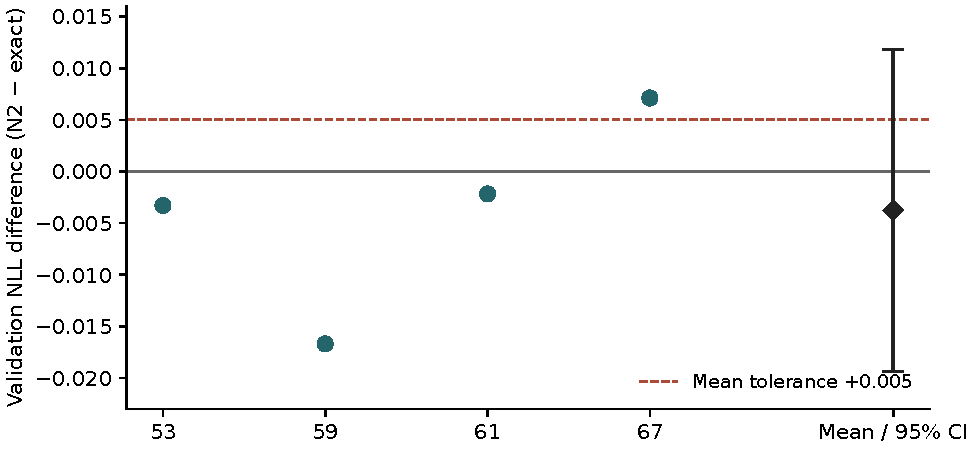
\includegraphics[width=.88\linewidth]{figures/quality_differences.pdf}
\caption{Paired endpoint differences and the mean's two-sided 95\% $t$ interval. The dashed line denotes the operational mean tolerance, not a per-seed acceptance threshold.}
\end{figure}

\subsection{A favorable raw-inverse comparison does not resolve the checkpointing comparison}
The original continuous-run throughput verdict was insufficient: its least favorable N2/N1 ratio was approximately 0.654, but measurement intervals included different I/O overheads. The matched throughput follow-up gives per-seed median ratios between 0.8418 and 0.8429. This resolves a specific timing mismatch against raw inversion; it does not imply an advantage over full checkpointing or erase the original verdict.

Likewise, memory figures require matching their windows. A learned-scale exact-reference checkpoint screen averages 20.609 GiB peak allocated memory, whereas continuous N2 training records approximately 11.706 GiB. Although the difference is large, these measurements come from different execution windows. We do not use that comparison as the decisive resource claim. Reserved memory and device-level usage also exceed allocated memory, so these numbers do not establish that the run fits a 12-GB GPU.

\subsection{Full checkpointing is stronger in matched resource probes}
At 4,096 tokens in the context ladder, a representative seed gives 11,375.7 tokens/s for full checkpointing and 8,358.7 for N2, with peak allocated memory of 11,909,809,664 and 11,951,753,216 bytes respectively. Across seeds, the mostly checkpointed K1 variant is about 1.35 times as fast as N2 at this length. Full checkpointing is slightly faster and smaller still in the recorded comparison.

The separate A800 measurements reach the same qualitative conclusion (Table~\ref{tab:a800}). At length 4,096, N2 reaches 71.65\% of full-checkpoint throughput and uses 0.33\% more peak allocated memory. At length 512, the corresponding figures are 71.30\% and 0.37\%. These short probes do not characterize sustained utilization, thermal behavior, or a broader kernel configuration space; they nevertheless contradict a general resource-dominance claim for the measured N2 implementation.

\begin{table}[ht]
\centering\small
\begin{tabular}{llrr}
\toprule Length & Backend & Allocated bytes & Tokens/s\\\midrule
512 & Full checkpoint & 11,774,053,888 & 13,305.4\\
512 & N2 & 11,818,094,592 & 9,486.3\\
4,096 & Full checkpoint & 11,795,025,408 & 12,102.8\\
4,096 & N2 & 11,834,347,520 & 8,672.1\\\bottomrule
\end{tabular}
\caption{A800 eager Flash-SDPA resource probes. Values are medians of three trials, each timing three training steps. These are descriptive summaries without inferential error bars.}
\label{tab:a800}
\end{table}
\begin{figure}[ht]
\centering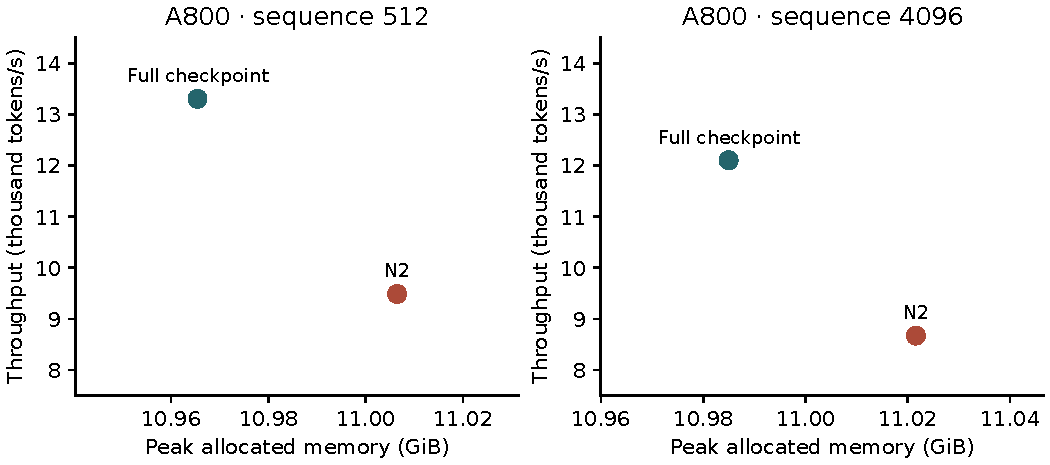
\includegraphics[width=\linewidth]{figures/a800_tradeoff.pdf}
\caption{The A800 measurements favor full checkpointing on both measured axes. The memory axis is intentionally expanded to show the small difference; absolute values remain approximately 11 GiB.}
\end{figure}

\subsection{The context continuation answers a narrower question}
Eight short continuations compare K1 and N2 at length 4,096: two methods across four seeds, with 1,003,520 additional tokens per run. The mean K1-minus-N2 validation loss is $+0.001278$, but one seed reaches $+0.005922$, exceeding the internal per-seed tolerance of $+0.005$. This motivated retaining N2 as the internal long-context default among those two candidates. It does not establish N2 as a better default than full checkpointing, which was not included in that continuation-quality comparison. Nor does a four-thousand-token continuation support a 128K-context claim.

\section{Limitations and release scope}
The experiments cover one hybrid architecture family, one corpus/tokenizer combination, and short training budgets. Four seed pairs are insufficient for a precise noninferiority conclusion. Shared seeds after checkpoint-based selection reduce independence, and operational tolerances were internally frozen rather than publicly preregistered. For the per-block learned-scale N2 method in the main study, we have not evaluated downstream tasks, pretrained-model conversion, PEFT or LoRA training, billion-token convergence, or broad hardware scaling. Later fixed-scale segmented variants have task-level and two-stack exploratory records, described separately in Appendix~\ref{app:later}; these do not fill the N2-specific evidence gaps.

The packaged N2 backend rejects frozen parameters in reversible blocks during gradient-enabled training, reflecting a limitation of the frozen backward implementation. Evaluation without gradients is supported. The CPU demonstration uses a small FP32 model and synthetic tokens to verify execution and checkpoint/resume behavior; it is not a reproduction of the historical GPU quality results. Local validation includes 11 passing checks covering installed-package execution, numeric paths, saved INT8 tensors, resume behavior, and rejection of unsupported frozen-parameter training. These checks establish software behavior within their scope, not scientific generality.

The manuscript is an evidence-audited working draft accompanying the source release at \url{https://github.com/Hldao/hui-reversible-research}. Before an academic submission, author/venue requirements and a complete historical environment and command manifest must be checked. Raw checkpoint accessibility, corpus redistribution constraints, and a clean independently executed GPU reproduction remain unresolved release items. No peer-reviewed acceptance or independent N2 50-million-token replication is claimed here. An older two-node short reproduction belongs to a different 124-million-parameter experiment and is not substituted for that missing evidence.

\section{Conclusion}
In Hui, quantized inverse-residual correction improves the observed numerical reliability of reversible backward computation. Its operationally acceptable four-seed endpoints do not establish statistical noninferiority, and the matched systems evidence favors full checkpointing over the current corrected implementation. The useful research object is therefore a transparent finite-precision case study with a reproducible implementation and explicit comparison boundaries. Further work should test independent seeds, sustained matched benchmarks, and broader tasks before making stronger quality or efficiency claims.

\appendix
\section{Reproducing the manuscript artifacts}
The draft includes audited numeric summaries, generated tables and statistics, and the script \path{build_results.py}. Running that script with Python and Matplotlib regenerates the figures and paired statistics; it does not rerun archived training. The core source SHA-256 digest (the following two lines concatenated) is:
\begin{quote}\ttfamily\small
87c78274e2bd6f9959d33b6e84d89351\\
176471cfd84936e2f99e106c807b87f1
\end{quote}
 Source provenance and packaging limitations are documented separately in the release candidate. Data-file hashes identify the audited token streams; they are not licenses to redistribute those streams.


\section{Later segmented variants and task-level evidence}
\label{app:later}
An expanded audit located later experiments from August 20--22 that were absent from the initial draft. They use a fixed-scale Hybrid75 model with 1,346,435,072 parameters, rather than the main study's 1,346,435,108-parameter learned-scale model. The 36-parameter difference is consistent with the main recipe's two learned scale logits in each of 18 reversible layers. Their segmented backward routes, packed 4-bit correction (C4), and group-wise 8-bit correction (C8 G1024) are distinct from per-block N2. They are exploratory extensions, not additional N2 seeds or interchangeable replications.

\subsection{Resource savings depend on the implementation and workload}
The v11 segmented experiment uses sequence length 4,096, batch eight, forced PyTorch Flash SDPA, and Liger fused linear cross-entropy 0.8.2. Three trials, each timing three updates, give C4 median allocated memory of 18,744,430,080 bytes versus 18,925,723,136 for the native full-checkpoint baseline. Median reserved memory is 19,549,650,944 versus 20,514,340,864 bytes; throughput is 11,845.9 versus 14,582.3 tokens/s (81.23\%). This is a small allocated-memory saving with a speed penalty. Batch size, loss backend, source recipe, and correction layout differ from the main N2 probe, so these results neither overturn its negative resource comparison nor establish a universal advantage.

\subsection{Short numerical agreement does not ensure downstream acceptance}
The v12 fresh-data screen passes its internal 64-update development criteria for C4. In the subsequent single-seed, 128-update synthetic structured-RAG experiment (v13), C4's held-out cross-entropy is 0.452376 versus 0.276117 for the full baseline, a difference of $+0.176259$. Its greedy all-fields accuracy is nevertheless higher (0.125 versus 0.083333 on 24 rows). The cross-entropy gate fails. A missing-dependency attempt is preserved with zero optimizer updates and excluded from valid-arm aggregation. Thus short numerical agreement, generation accuracy, and cross-entropy are separate acceptance dimensions. This synthetic task does not establish general natural-language RAG quality.

\subsection{Backend, learning rate, and horizon can change the ranking}
A subsequent development factorial selects a C4-to-C8 schedule and a reduced learning rate on the same 24 rows; this selection requires fresh confirmation. The later two-stack synthetic confirmation accepts the candidate on A800/CUDA but rejects it on S4000/MUSA. The latter also requires an arithmetic repair for an unsupported C4 bit-shift operator. A successful compatibility repair does not itself establish quality parity.

A separate fixed-evidence public-proxy QA factorial (v27) controls learning rate within each backend. Table~\ref{tab:later} shows all four matched route effects at 128 updates. The candidate is the scheduled segmented C4-to-C8 route, not N2. The sign changes across backend at the original learning rate. These are one-seed local effects on one physical device per stack; they do not support hardware-wide generalization or comparisons that confound route with learning rate. Supplied evidence is fixed; this is not an evaluation of document retrieval.
\begin{table}[ht]
\centering
\begin{tabular}{llrrr}
\toprule Stack & LR multiplier & Full CE & Candidate CE & Difference\\\midrule
CUDA & 0.75 & 6.911331 & 6.942330 & +0.030998\\
CUDA & 1.00 & 6.878812 & 6.955012 & +0.076200\\
MUSA & 0.75 & 6.966712 & 6.985117 & +0.018405\\
MUSA & 1.00 & 6.949034 & 6.901833 & -0.047200\\\bottomrule
\end{tabular}
\caption{Exploratory same-learning-rate route comparisons at 128 updates. Positive differences indicate higher candidate cross-entropy. Developmental thresholds are not statistical noninferiority tests.}
\label{tab:later}
\end{table}

At 256 updates in later same-corpus continuations, candidate-minus-full CE is $-0.003028$ on A800 (v33) and $-0.036858$ on S4000 (v35). These point estimates do not establish superiority: for example, the S4000 row-bootstrap interval at the endpoint is $[-0.091008,+0.018093]$. Such resampling describes the fixed evaluation rows, not uncertainty across training seeds. At S4000 step 192, the difference is instead $+0.025407$, illustrating horizon sensitivity. The failed S4000 parent run could not attest embedding-adapter restoration and is excluded; the corrected full arm was rerun. Historical labels containing ``noninferior'' or ``better'' remain operational labels, not statistical conclusions.

\subsection{Migration canary and its boundary}
A separate operational canary (v39) records per-backend exact-at-load fresh-process resume and portable CPU-strict export reload checks on one A800 and one S4000. The source checkpoint and training-data hashes agree. A terminal set opened after both exports contains only 36 rows and 175 target tokens. Terminal target-token accuracy is 0.400000 and 0.405714; mean target CE is 4.242752 and 4.027876, respectively. These are descriptive canary outcomes. They do not establish arbitrary cross-device optimizer-trajectory equivalence, an independent N2 replication, production quality, or active route control.

\section{Expanded audit coverage}
The local inventory covers 25 evidence directories, including data packs and earlier audit outputs; this is not a count of independent experiments. For the extensions above, 30 recorded input-hash links were checked against result files, nine v11 resource trials were reaggregated, and v13, v27, v33, v35, and v39 headline metrics were checked against underlying receipts. Forty-nine local source files are identified by digest in the accompanying extended-audit summary; recovered NAS source excerpts provide additional arithmetic provenance. This record audit does not rerun GPU training or rehash all raw checkpoints. Later implementation slices remain outside the minimal source release.

\clearpage
\bibliographystyle{plain}
\bibliography{references}
\end{document}
